\subsection{Round 1 Problems}

Solutions can be found in Section~\ref{S::2024-S-1}.

\mcq

\begin{enumerate}
    \hyperrefitem[Q::2024-S-1-1] Find the largest positive integer $A$ such that $2^x + \dfrac{2025}{2^x} - A > 0$ for all real numbers $x$
    \begin{tasks}(5)
        \task 59
        \task 69
        \task 79
        \task 89
        \task 99
    \end{tasks}
    \hyperrefitem[Q::2024-S-1-2] If $x = \dfrac{1}{\log_{\frac{2024}{2023}} 7} + \dfrac{1}{\log_{\frac{2023}{2022}} 7} + \dfrac{1}{\log_{\frac{2022}{2021}} 7}$, find $7^x$.
    \begin{tasks}(5)
        \task $\dfrac{2021}{2024}$
        \task $\dfrac{2024}{2021}$
        \task $\dfrac{2022}{2024}$
        \task $\dfrac{2024}{2022}$
        \task $2024$
    \end{tasks}
    \hyperrefitem[Q::2024-S-1-3] Simplify $\dfrac{2024}{\sqrt{4 + \sqrt{12}}} + \dfrac{2024}{\sqrt{4 - \sqrt{12}}}$.
    \begin{tasks}(5)
        \task 1012
        \task $1012\sqrt3$
        \task 2024
        \task $2024\sqrt3$
        \task! $1012 + 1012\sqrt3$
    \end{tasks}
    \hyperrefitem[Q::2024-S-1-4] Suppose $x^{1/3} + 12 = y^{1/3}$ for some real numbers $x$ and $y$. Find the minimum possible value of $y-x$.
    \begin{tasks}(5)
        \task 432
        \task 532
        \task 632
        \task 732
        \task! None of the above
    \end{tasks}
    \hyperrefitem[Q::2024-S-1-5] Find the largest possible value of $\dfrac{\sqrt2 \cos{2x}}{\sin{x} + \cos{x}}$.
    \begin{tasks}(5)
        \task $\dfrac12$
        \task 1
        \task $\dfrac32$
        \task 2
        \task $\dfrac52$
    \end{tasks}
\end{enumerate}

\sq

\begin{enumerate}
    \setcounter{enumi}{5}
    \hyperrefitem[Q::2024-S-1-6] If $\sqrt{x + \sqrt{x}} + \sqrt{x - \sqrt{x}} = 4$, find the value of $15x$.
    \hyperrefitem[Q::2024-S-1-7] Find the smallest positive integer $K$ such that \[x^2 - 200x + y^2 = 0 \text{ and } x + y \leq K.\]
    \hyperrefitem[Q::2024-S-1-8] Given that $\dfrac{\cos{x}}{\sin{3x}} - \dfrac{\sin{x}}{\cos{3x}} - 2 \cdot \dfrac{\sin{4x}}{\cos{6x}} = 2024$, find the value of $\dfrac{\cos{10x}}{\sin{12x}}$.
    \hyperrefitem[Q::2024-S-1-9] Find the smallest positive integer $k$ such that the coefficient of $x^k$ in the expansion of $\bp{5x^3 + \frac1{\sqrt{x}}}^{2024}$ is \textbf{not} zero.
    \hyperrefitem[Q::2024-S-1-10] Let \[P = \bp{2024^2 + 1}\bp{2024^{2^2} + 1}\bp{2024^{2^3} + 1}\cdots\bp{2024^{2^{10}} + 1} \times 2025 + \dfrac1{2023}.\] Find the smallest positive integer $N$ such that $N > \log_{2024} P$.
    \hyperrefitem[Q::2024-S-1-11] Let $\triangle ABC$ be a triangle with area 1000. Let $M$ and $N$ be points on $AB$ and $AC$ respectively such that \[AM : MB = 3 : 2 \text{ and } AN : NC = 7 : 3.\] Let $X$ and $Y$ be the midpoints of $BN$ and $CM$ respectively. Find the area of $\triangle AXY$.

    \begin{center}
        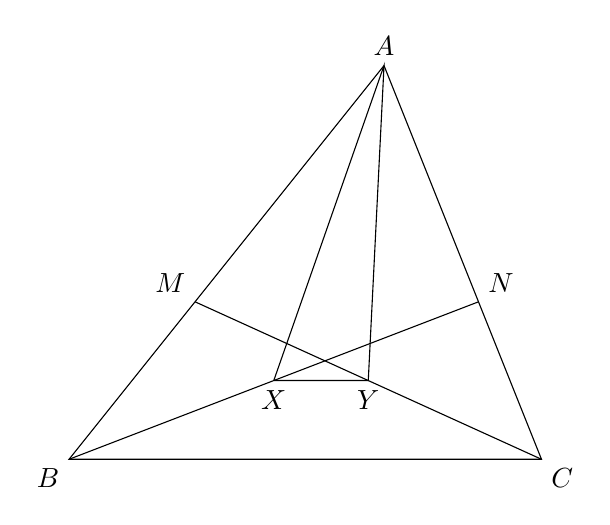
\begin{tikzpicture}
            \coordinate[label=above:$A$] (A) at (4, 5);
            \coordinate[label=below left:$B$] (B) at (0, 0);
            \coordinate[label=below right:$C$] (C) at (6, 0);
            \coordinate[label=above left:$M$] (M) at (1.6, 2);
            \coordinate[label=above right:$N$] (N) at (5.2, 2);
            \coordinate[label=below:$X$] (X) at (2.6, 1);
            \coordinate[label=below:$Y$] (Y) at (3.8, 1);

            \draw (A) -- (B) -- (C) -- (A);

            \draw (C) -- (M);
            \draw (B) -- (N);
            
            \draw (X) -- (A) -- (Y) -- (X);
        \end{tikzpicture}
    \end{center}
    \hyperrefitem[Q::2024-S-1-12] Find the largest positive integer $n \leq 10000$ such that $1 + 2024n^2$ is a perfect square.
    \hyperrefitem[Q::2024-S-1-13] In a tetrahedron $SABC$, the faces $SBC$ and $ABC$ are perpendicular to each other. The angles $\angle ASB$, $\angle BSC$, $\angle ASC$ are all $60\deg$, and $SB = SC = 4$. Find the square of the volume of the tetrahedron.

    \begin{center}
        \begin{tikzpicture}[scale=0.8]
            \coordinate[label=left:$A$] (A) at (-1.5, 2);
            \coordinate[label=below:$B$] (B) at (0, 0);
            \coordinate[label=right:$C$] (C) at (5, 2);
            \coordinate[label=above:$S$] (S) at (3, 6);

            \draw (A) -- (B) -- (C) -- (S) --  (A);
            \draw[dashed] (A) -- (C);
            \draw (S) -- (B);
        \end{tikzpicture}
    \end{center}
    \hyperrefitem[Q::2024-S-1-14] Let $a$, $b$, $c$ be the three real roots of the cubic equation \[2x^3 - 4x^2 - 21x - 8 = 0.\] Given that \[S = \frac1{ab + c -1} + \frac1{bc + a -1} + \frac1{ca + b - 1}\] is a rational number that can be expressed as a fraction in the lowest form $\frac{m}{n}$, find the value of $m^2 + n^2$.
    \hyperrefitem[Q::2024-S-1-15] Consider the equation \[\frac{\sqrt3 - 1}{\sin x} + \frac{\sqrt3 + 1}{\cos x} = 4\sqrt2.\] For the range $0 < x < \pi/2$, the sum of the solutions of the equation can be expressed in the form $\frac{m\pi}{n}$, where $\frac{m}{n}$ is a fraction in the lowest form. Find $m + n$.
    \hyperrefitem[Q::2024-S-1-16] An engineer constructs a circle with centre $O$ and diameter $CD$ on level ground, and builds a vertical tower of height 20 at the centre. $B$ is another point on the circumference and $P$ is on $CD$ produced such that $PB$ is a secant line of the circle. Given that $PB = 33$, $PC = 77$ and $CD = 74$, find the minimum possible distance of any point on $PB$ to the top of the tower.

    \begin{center}
        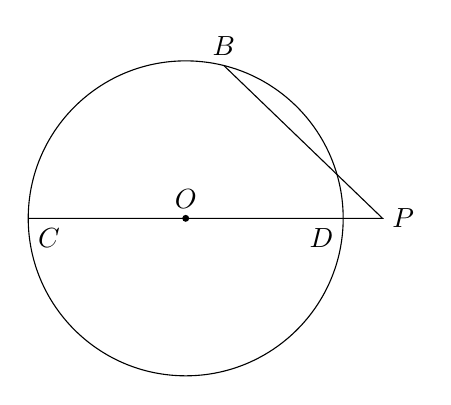
\begin{tikzpicture}[scale=0.5]
            \coordinate[label=above:$B$] (B) at (0.97, 3.88);
            \coordinate[label=right:$P$] (P) at (5, 0);
            \coordinate[label=below right:$C$] (C) at (-4, 0);
            \coordinate[label=below left:$D$] (D) at (4, 0);
            \coordinate[label=above:$O$] (O) at (0, 0);

            \draw (C) -- (P) -- (B);

            \draw (O) circle[radius=4];

            \fill (O) circle[radius=2.5pt];
        \end{tikzpicture}
    \end{center}
    \hyperrefitem[Q::2024-S-1-17] $P$ is a common point of tangency of two circles. $BA$ is a chord of the larger circle which is tangent to the smaller circle at a point $C$. $PB$ and $PA$ intersect the smaller circle at points $E$ and $D$ respectively. If $BA = 15$, $PE = 2$, and $PD = 3$, find the length $CA$.

    \begin{center}
        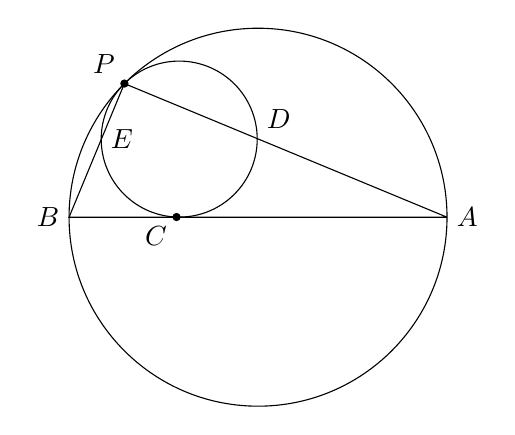
\begin{tikzpicture}[scale=0.3]
            \coordinate[label=right:$A$] (A) at (8, 0);
            \coordinate[label=left:$B$] (B) at (-8, 0);
            \coordinate[label=below left:$C$] (C) at (-3.45, 0.007);
            \coordinate[label=above right:$D$] (D) at (-0.035, 3.33);
            \coordinate[label=right:$E$] (E) at (-6.64, 3.29);
            \coordinate[label=above left:$P$] (P) at (-5.657, 5.657);
    
            \draw (0, 0) circle[radius=8];
            \draw (-3.337, 3.307) circle[radius=3.302];
            
            \draw (A) -- (B) -- (P) -- (A);
            \fill (P) circle[radius=5pt];
            \fill (C) circle[radius=5pt];
        \end{tikzpicture}
    \end{center}
    \hyperrefitem[Q::2024-S-1-18] On each face of a cube, an integer greater than 2 is written. Each vertex of the cube is the intersection of three unique faces, and each edge is the intersection of two unique faces. Assign to each vertex the product of the numbers written on the faces intersecting the vertex, and assign to each edge the product of the numbers written on the faces intersecting the edge. The sum of the numbers assigned to the eight vertices is equal to 2024. Find the maximum possible value of an edge.
    \hyperrefitem[Q::2024-S-1-19] Find the sum of the squares of each of the roots of the equation \[x^2 - 4\floor{x} - 12 = 0,\] where $\floor{x}$ denotes the greatest integer less than or equal to $x$.
    \hyperrefitem[Q::2024-S-1-20] Calculate the remainder when $1901^{2024}$ is divided by 1216.
    \hyperrefitem[Q::2024-S-1-21] Let $P(x) = a_0 + a_1 x + a_2 x^2 + \cdots + a_n x^n$ be a polynomial with non-negative integer coefficients satisfying $0 \leq a_i \leq 17$ for all $i$. If $P(18) = 367616$, find the value of $P(3)$.
    \hyperrefitem[Q::2024-S-1-22] Evaluate the sum \[\frac{2}{1 + \tan{\frac{\pi}{260}}} + \frac{2}{1 + \tan{\frac{2\pi}{260}}} + \frac{2}{1 + \tan{\frac{3\pi}{260}}} + \cdots + \frac{2}{1 + \tan{\frac{129\pi}{260}}}.\]
    \hyperrefitem[Q::2024-S-1-23] An equilateral triangle $ABC$ is inscribed in a circle and $P$ is a point on the minor arc $BC$. Point $D$ is the intersection of $AP$ and $BC$.

    \begin{center}
        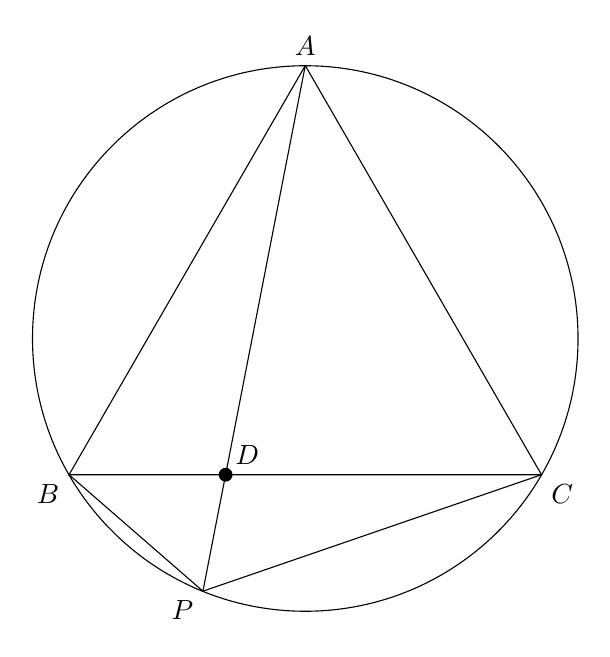
\begin{tikzpicture}
            \coordinate[label=above:$A$] (A) at (0, 5.196);
            \coordinate[label=below left:$B$] (B) at (-3, 0);
            \coordinate[label=below right:$C$] (C) at (3, 0);
            \coordinate[label=above right:$D$] (D) at (-1.011,0);
            \coordinate[label=below left:$P$] (P) at (-1.3, -1.479);
    
            \draw (A) -- (B) -- (C) -- (A);
            \draw (A) -- (P);
            \fill (D) circle[radius=2.5pt];
    
            \draw (0, 1.73) circle[radius=3.464];
            \draw (B) -- (P) -- (C);
        \end{tikzpicture}
    \end{center}

    Suppose that $BP = 5$, $CP = 20$. Find the length of $AD$.
    \hyperrefitem[Q::2024-S-1-24] Find the number of positive integers $x < 9000$ such that $x^3 + 95$ is divisible by 96.
    \hyperrefitem[Q::2024-S-1-25] A scalene triangle $\triangle ABC$ has sides $AB = 7$, $AC = 12$ and $BC = 13$. Write $\tan \frac{A-B}{2} \tan \frac{C}{2}$ as a fraction $\frac{m}{n}$ in its lowest form and find $m + n$.

    \begin{center}
        \begin{tikzpicture}[scale=0.5]
            \coordinate[label=above:$A$] (A) at (2.85, 6.40);
            \coordinate[label=below right:$B$] (B) at (13, 0);
            \coordinate[label=below left:$C$] (C) at (0, 0);
    
            \draw (A) -- (B) -- (C) -- (A);
    
            \node[anchor=south west] at ($(A)!0.5!(B)$) {7};
            \node[anchor=north] at ($(B)!0.5!(C)$) {13};
            \node[anchor=south east] at ($(C)!0.5!(A)$) {12};
        \end{tikzpicture}
    \end{center}
\end{enumerate}
